\begin{multicols}{2}[\section{Bachelor Wirtschaftsmathematik}]

Der Bachelor Wirtschaftsmathematik ist durch die Fachspezifischen Bestimmungen
(FSB) in einen mathematischen, einen wirtschaftlichen und einen Praxisbezogenen
Bereich gegliedert, in denen ihr bestimmte Leistungen erbringen müsst. In einem
vierten Bereich könnt ihr euer Studium nach euren Vorstellungen ausbauen, indem
ihr einen oder mehrere obligatorische Bereiche vertieft oder einfach etwas ganz
anderes macht! Wir stellen euch im folgenden diese vier Bereich vor.

\paragraph{Mathematik}

\subparagraph{Reine Mathematik}

Die Veranstaltungen in \emphm{Analysis I und II} und \emphm{Lineare Algebra \&
Analytische Geometrie I und II} müssen besucht werden. Um die Module zu
bestehen, müssen alle Teilmodulprüfungen bestanden werden. Diese sind regelhaft
als eine Klausur am Ende des zweiten Semesters zu absolvieren.

\emphm{Höhere Analysis} kann von euch idealerweise im dritten Semester als
mathematisches Vertiefungsmodul eingebracht werden.

\subparagraph{Angewandte Mathematik}

Dazu gehören \emphm{Numerische Mathematik} und \emphm{Mathematische
Stochastik}. Diese beiden Module finden regelhaft als 6 SWS Veranstaltungen im
dritten Semester statt und auch hier müsst ihr die Prüfungen bestehen.

Zum mathematischen Pflichtbereich gehören noch zwei Seminare. Ein Proseminar,
das auf einem Pflichtmodul aufbaut, und ein Seminar, das sich auf ein
mathematisches Vertiefungsmodul bezieht. Auf dieses Seminar kann dann eine
Bachelorarbeit aufgebaut werden.

\paragraph{Wirtschaftswissenschaften}

\subparagraph{Betriebswirtschaftslehre}

Als Pflichtmodule sind hier die beiden Vorlesungen \emphm{Investition} und
\emphm{Finanzierung} vorgesehen.  Zusätzlich könnt ihr weiterführende
betriebswirtschaftliche Vorlesungen als wirtschaftliche Wahlmodule wählen. Dazu
gibt es folgende Auswahl:

\begin{itemize}\itemsep 0pt
    \item Bilanzen (6 LP)
    \item Einführung ins Marketing (6 LP)
    \item Grundlagen der Wirtschaftsinformatik (6 LP)
    \item Grundlagen Rechnungswesen (6 LP)
    \item Kosten-Leistungsrechnung (3 LP)
    \item Produktion (6 LP)
\end{itemize}

Zudem sind betriebswirtschaftliche Vertiefungsmodule aus folgenden Bereichen zu
wählen: 

% TODO: LP
\begin{itemize}\itemsep 0pt
    \item Finanzen und Versicherungen
    \item Marketing und Medien
    \item Operational Management und Logistik
    \item Wirtschaftsinformatik
\end{itemize}

\subparagraph{Volkswirtschaftslehre}

Als Pflichtmodule sind hier die beiden Vorlesungen \emphm{Mikroökonomie} und
\emphm{Makroökonomie} vorgesehen. Auch in diesem Bereich gibt es einige
wirtschaftliche Wahlmodule, die ihr belegen könnt:

\begin{itemize}\itemsep 0pt
    \item Außenwirtschaftslehre (6 LP)
    \item Finanzwissenschaft (6 LP)
    \item Industrieökonomik (6 LP)
    \item Ökonometrie (12 LP)
\end{itemize}

Im Anschluss können hier ebenso Vertiefungsmodule im Rahmen von 12 LP besucht
werden.

Im wirtschaftlichen Bereich muss ein gewisser Anteil von LP mit mindestens
einem Seminar abgedeckt werden. Für ein Seminar muss meist zuvor die zugehörige
Vorlesung gehört werden.

\paragraph{Allgemeine Berufsqualifizierende Kompetenzen}

Genau wie die Studenten des Studiengangs Bachelor Mathematik müsst ihr drei
Module zu Allgemeine Berufsqualifizierende Kompetenzen (ABK) belegen. Dazu
gehört das Modul \emphm{Programmiermethoden}, welches hilfreich für die
Vorlesung \emphm{Numerische Mathematik} ist. Dieses Modul wird immer in
der vorlesungsfreien Zeit angeboten. In diesem Modul und im Modul
\emphm{Softwarepraktikum} müsst ihr jeweils die Modulprüfung bestehen.

Da das Bachelorstudium praxisnäher sein soll, müsst ihr ein ABK-Modul von 5 LP
absolvieren, entweder als Betriebspraktikum, als Projektarbeit oder als
Tutorium für Übungspruppen.

\paragraph{Wahlmodule}

Im Laufe des Bachelorstudienganges müsst ihr 6 LP an Wahlmodulen belegen. Diese
sollten nicht zu früh belegt werden, da ihr erst einmal im Pflichtbereich den
Uni-Alltag kennenlernen solltet, um euch einen Überblick zu verschaffen. Die
Module können aus dem kompletten Katalog der Universität, zuzüglich der TU
Hamburg-Harburg gewählt werden. Daher solltet ihr auf eine sinnvolle Ergänzung
eures Studiums achten.

\begin{center}
\vfill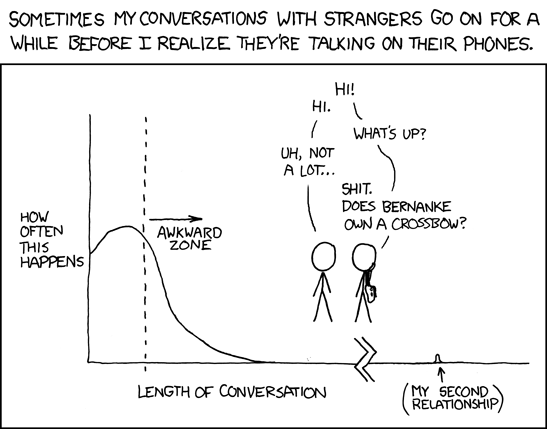
\includegraphics[scale=.55]{comics/476}
\end{center}

\end{multicols}

\clearpage

\subsection{Musterstudienplan für den Studiengang B.Sc.  Wirtschaftsmathematik
- Variante BWL}

\begin{center}
\begin{tabular}{||l||l|l|l|l|l|l||}
\hhline{|t:=:t:=t=t=t=t=t=:t|}
\hspace*{25mm}&1. Semester\hspace*{8ex}&2. Semester\hspace*{8ex}&3. Semester\hspace*{8ex}&4.Semester\hspace*{8ex}&5. Semester\hspace*{8ex}&6. Semester\hspace*{8ex}\\
\hhline{|:=::======:|} Pflichtbereich&Analysis I&Analysis II&Mathematische& Proseminar &Seminar& Bachelorarbeit\\
\hhline{||~||~|~|~|~|~|~||} Mathematik &(9 LP)&(9 LP)&Stochastik&(4 LP) &(6 LP)& (12 LP)\\
\hhline{||~||~|~|~|~|~|~||} &&&(9 LP)&&&\\
\hhline{||~||~|~|~|~|~|~||} &Lineare Algebra&Lineare Algebra&&&&\\ 
\hhline{||~||~|~|~|~|~|~||} &und Analytische &und Analytische&Numerische& & &\\ 
\hhline{||~||~|~|~|~|~|~||} &Geometrie I&Geometrie II&Mathematik&&&\\ 
\hhline{||~||~|~|~|~|~|~||} &(9 LP)&(9 LP)&(9 LP)&&&\\
\hhline{||~||~|~|~|~|~|~||} &&&&&&\\
\hhline{|:=::======:|} Pflichtbereich&Investition&Finanzierung&&Mikroökonomik&Makroökonomik&\\
\hhline{||~||~|~|~|~|~|~||} Wirtschaft  &  (6 LP)  &(6 LP) &   &(6 LP) &  (6 LP)  &\\
\hhline{||~||~|~|~|~|~|~||} &&&&&&\\
\hhline{|:=::======:|} Wahlpflichtbereich&&&&Vertiefungsmodule&Vertiefungsmodule&Vertiefungsmodule \\
\hhline{||~||~|~|~|~|~|~||} Mathematik&&&&(11 LP)&(7 LP)&(9 LP)\\
\hhline{||~||~|~|~|~|~|~||} &&&&&&\\
\hhline{|:=::=|=|=|=|=|=:|} Wahlpflichtbereich&Wahlpflichtmodule&&Wahlpflichtmodule &Wahlpflichtmodule&Vertiefungsmodule&Vertiefungsmodule \\
\hhline{||~||~|~|~|~|~|~||} Wirtschaft&(6 LP)&&(6 LP)&(9 LP)&(6 LP)&(6 LP)\\
\hhline{||~||~|~|~|~|~|~||} &&&&&&\\
\hhline{|:=::======:|} ABK-Bereich&&Programmier-&Softwarepraktikum&&Betriebspraktikum/& \\
\hhline{||~||~|~|~|~|~|~||} &&methoden&(4 LP)&&Projekt/Tutorium&\\
\hhline{||~||~|~|~|~|~|~||} &&(5 LP)&&&(5 LP)&\\
\hhline{||~||~|~|~|~|~|~||} &&&&&&\\
\hhline{|:=::======:|} Wahlbereich&&Wahlmodule&Wahlmodule&&&Wahlmodule\\
\hhline{||~||~|~|~|~|~|~||} &&(1 LP)&(2 LP)&&&(3 LP)\\
\hhline{||~||~|~|~|~|~|~||} &&&&&&\\
\hhline{|b:=:b:======:b|}
\end{tabular}
\end{center}

\clearpage

\subsection{Musterstudienplan für den Studiengang B.Sc.-Wirtschaftsmathematik -
Variante VWL}

\begin{center}
\begin{tabular}{||l||l|l|l|l|l|l||}
\hhline{|t:=:t:=t=t=t=t=t=:t|}
\hspace*{25mm}&1. Semester\hspace*{8ex}&2. Semester\hspace*{8ex}&3. Semester\hspace*{8ex}&4.Semester\hspace*{8ex}&5. Semester\hspace*{8ex}&6. Semester\hspace*{8ex}\\
\hhline{|:=::======:|} Pflichtbereich&Analysis I&Analysis II&Mathematische&Proseminar&Seminar&Bachelorarbeit\\
\hhline{||~||~|~|~|~|~|~||} Mathematik &(9 LP)&(9 LP)&Stochastik&(4 LP)&(6 LP)& (12 LP)\\
\hhline{||~||~|~|~|~|~|~||} &&&(9 LP)&&&\\
\hhline{||~||~|~|~|~|~|~||} &Lineare Algebra&Lineare Algebra&&&&\\ 
\hhline{||~||~|~|~|~|~|~||} &und Analytische&und Analytische&Numerische&&&\\ 
\hhline{||~||~|~|~|~|~|~||} &Geometrie I&Geometrie II&Mathematik&&&\\ 
\hhline{||~||~|~|~|~|~|~||} &(9 LP)&(9 LP)&(9 LP)&&&\\
\hhline{||~||~|~|~|~|~|~||} &&&&&&\\
\hhline{|:=::======:|} Pflichtbereich&Investition&Mikroökonomie&Makroökonomik&Finanzierung&&\\
\hhline{||~||~|~|~|~|~|~||} Wirtschaft&(6 LP)&(6 LP)&(6 LP)&(6 LP)&&\\
\hhline{||~||~|~|~|~|~|~||} &&&&&&\\
\hhline{|:=::======:|} Wahlpflichtbereich&&&&Vertiefungsmodule&Vertiefungsmodule&Vertiefungsmodule\\
\hhline{||~||~|~|~|~|~|~||} Mathematik&&&&(11 LP)&(7 LP)&(9 LP)\\
\hhline{||~||~|~|~|~|~|~||} &&&&&&\\
\hhline{|:=::======:|} Wahlpflichtbereich&Wahlpflichtmodule&&&Wahlpflichtmodule&Wahlpflichtmodule&\\
\hhline{||~||~|~|~|~|~|~||} Wirtschaft&(6 LP)&&&(9 LP)&(6 LP)&\\
\hhline{||~||~|~|~|~|~|~||} &&&&&&\\
\hhline{||~||~|~|~|~|~|~||} &&&&&Vertiefungsmodule&Vertiefungsmodule\\
\hhline{||~||~|~|~|~|~|~||} &&&&&(6 LP)&(6 LP)\\
\hhline{||~||~|~|~|~|~|~||} &&&&&&\\
\hhline{|:=::======:|} ABK-Bereich&&Programmier-&Softwarepraktikum&&Betriebspraktikum/&\\
\hhline{||~||~|~|~|~|~|~||} &&methoden&(4 LP)&&Projekt/Tutorium&\\
\hhline{||~||~|~|~|~|~|~||} &&(5 LP)&&&(5 LP)&\\
\hhline{||~||~|~|~|~|~|~||} &&&&&&\\
\hhline{|:=::======:|} Wahlbereich&&Wahlmodule&Wahlmodule&&&Wahlmodule\\
\hhline{||~||~|~|~|~|~|~||} &&(1 LP)&(2 LP)&&&(3 LP)\\
\hhline{||~||~|~|~|~|~|~||} &&&&&&\\
\hhline{|b:=:b:======:b|}
\end{tabular}
\end{center}
\clearpage
